\section{Profile Select Activity}
This section will explain the profile select activity and how it makes some of the external architecture for others to use.

The final implementation of the design is made so it is simple and easy to use. 

This can be seen in \autoref{fig:profile-select-activity_2} and in \autoref{fig:profile-select-activity_1} on page \pageref{fig:profile-select-activity_1}.

\begin{figure}[h!]
	\centering
	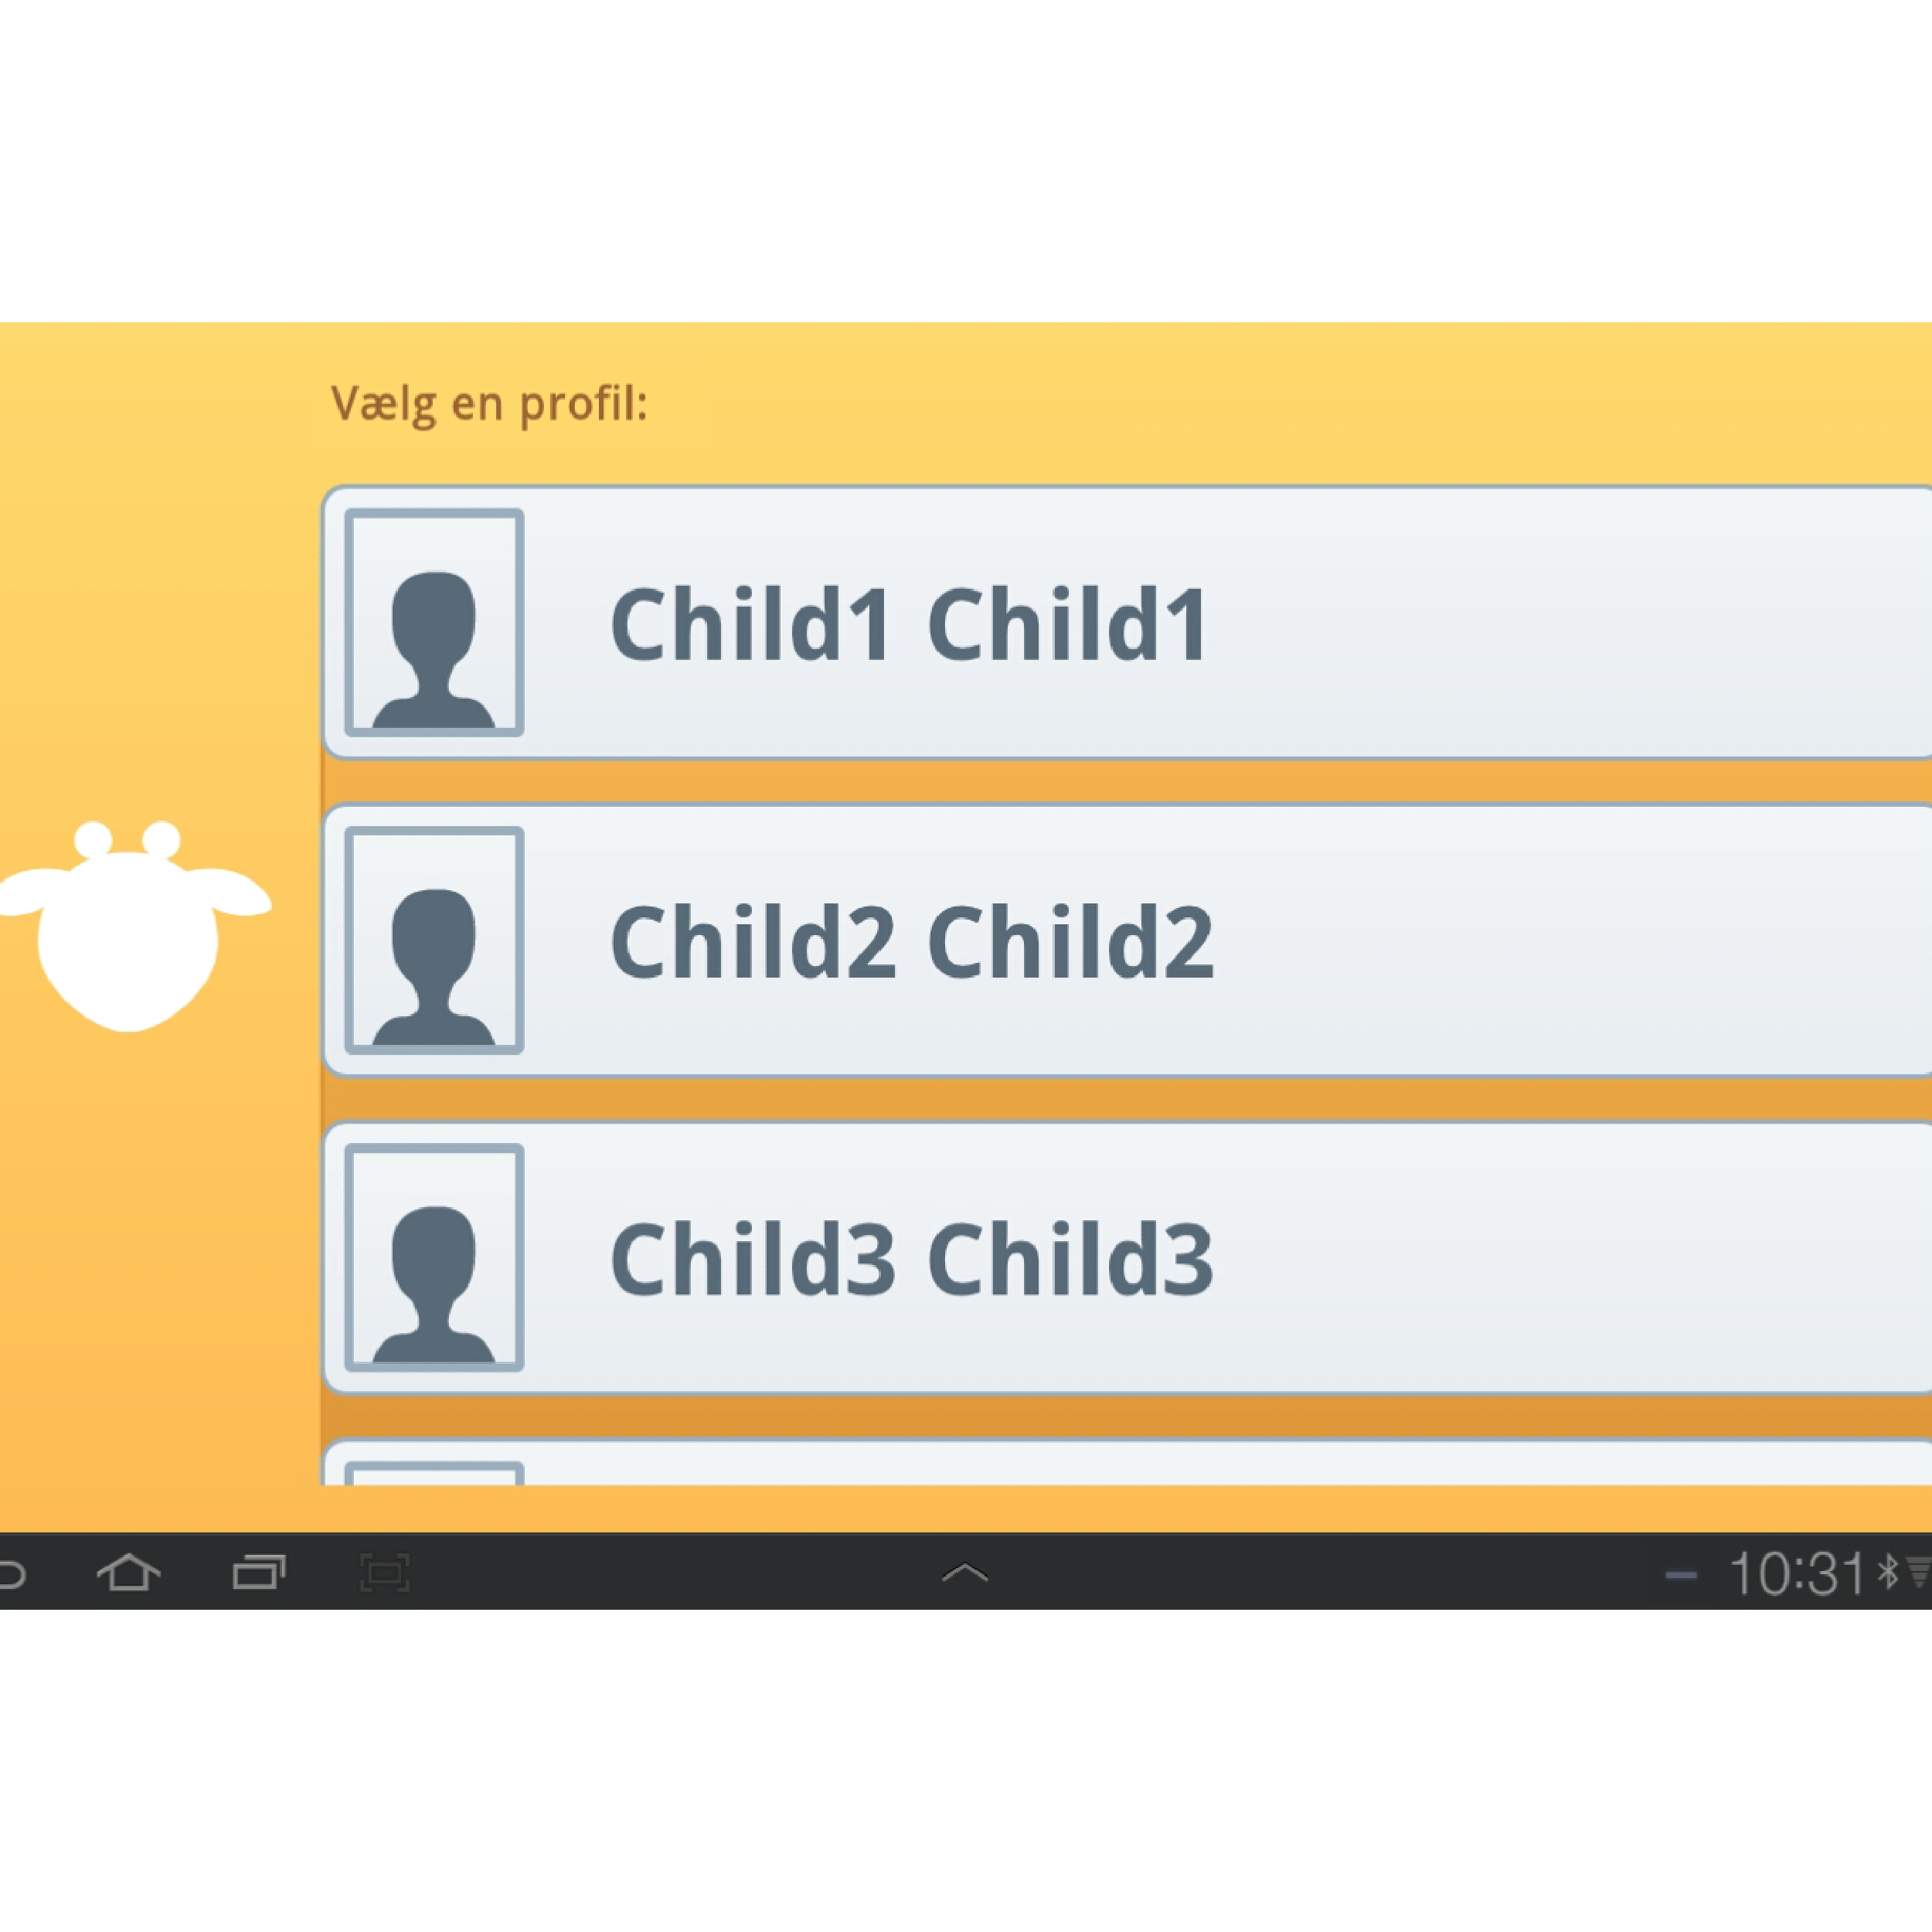
\includegraphics[scale=0.3]{gfx/profile-select-activity_2.jpg}
	\caption{Landscape profile select activity screenshot}
	\label{fig:profile-select-activity_2}
\end{figure}

\begin{lstlisting}[style=sourceCode, language=JAVA, caption=How the launcher shares different ids and color through the profile select activity, label=lst:profileActivity] 
listOfChildren.setOnItemClickListener(new OnItemClickListener() {
			public void onItemClick(AdapterView<?> parent, View view, int position, long id) {
				final long childID = ((Profile) parent.getAdapter().getItem(position)).getId();

				Intent intent = new Intent(Intent.ACTION_MAIN);
				intent.addCategory(Intent.CATEGORY_LAUNCHER);
				intent.setComponent(new ComponentName(mPackageName, mActivityName));
				intent.setFlags(Intent.FLAG_ACTIVITY_NEW_TASK
						| Intent.FLAG_ACTIVITY_RESET_TASK_IF_NEEDED);

				intent.putExtra(Data.CHILDID, childID);
				intent.putExtra(Data.GUARDIANID, mGuardianID);
				intent.putExtra(Data.APP_COLOR, mAppColor);

				startActivity(intent);
			}
		});
\end{lstlisting}